\section{PVS model}
We will now discuss how the PVS model looks like, from the datatypes used to the abstractions applied. Furthermore, we will show how the original C++ source code was converted to PVS and what problems occured. Where possible, we will use excerpts of the model to help clarify the text. While discussing our model, it is important that one keeps in mind that our verification attempts only look at IPC from the perspective of the current thread.

\subsection{Properties}
As our model has been created with the properties we wanted to prove in mind, we will first discuss those properties. We have looked at three different properties, each of which we will now discuss in more detail.

\subsubsection{Property 1: removal of sender's thread lock on receiver}
Before a sender can send a message to a receiver, they both have to agree upon engaging in IPC (referred to as the \emph{handshake}). The message can only be sent if the handshake is successful. When sending a message, the sender has to make sure that the receiver thread is not locked by another thread. If it is, the sender will acquire a thread lock on the receiver before sending the message. After the sending has finished, any acquired thread lock on the receiver should be released as otherwise no other threads can access the receiver subsequently.

\subsubsection{Property 2: waking up receiver in combined send/receive}
As explained earlier, it is possible to make a combined send- and receive IPC call. This means that after having sent its message to the receiver, the sender then waits for the receiver to send a message back. Essentially this means that after the first message is sent, the sender- and receiver roles are swapped. At the moment where the receiver assumes the sender role, it should be ready to be scheduled (in other words, the receiver is awoken). If the receiver is not ready to be scheduled when the roles are swapped, it might never be scheduled again, which might result in the sender waiting forever to receive a message back.

\subsubsection{Property 3: validation of assertions in the code}
In the Fiasco C++ source code, there are several calls to the \emph{assert()} function. Basically, a call to \emph{assert()} is meant to ensure that the system is in a correct state. The \emph{assert()} function takes a boolean expression as its parameter, which it evaluates. If the expression evaluates to true, execution is continued normally. However, if the expression evaluates to false, execution of the program is aborted. Assertions should thus only be used when a specific condition \textit{has} to hold. As we have included the assertions in our model, we tried to verify that all assert calls evaluate to true. If we could verify this, that would give us some confidence in the correctness of our model.

\subsection{Abstractions}
To prevent the model and proofs from becoming too complex, we abstracted away many parts of Fiasco IPC. The abstractions depend in part on the above-mentioned properties, but also on the complexity of some parts of IPC. We will now list the most important abstractions:

\begin{itemize}
 \item \textbf{Implementation of functions}: in some cases we kept the model simple by hiding the implementation of specific functions. In these cases we were only interested in \textit{what} the effect of a function was, not on \textit{how} it was achieved.
 \item \textbf{Different senders}: of the three possible IPC message senders, we have only modelled one: threads. The preemption- and interrupt IPC message senders have been abstracted away as inclusion would have required two additional send paths to be added to the model.
 \item \textbf{Scheduling}: we are not interested in \textit{how} and \textit{which} threads are scheduled, our only concern is with the effect this scheduling has on IPC. Anything related to scheduling, such as the execution- and scheduling context concepts, is thus not included in our model.
 \item \textbf{Receive part}: the properties we looked at mostly concerned the send part of IPC, which resulted in the abstraction of the receive part. The receive part does appear in a slightly modified form in our preemption point implementation.
 \item \textbf{Long IPC}: in contrast to the short IPC path, the long IPC path is fully interruptible. This greatly increases the complexity, as the system can interrupt ongoing IPC at any time. Furthermore, in long IPC page-faults can occur which require special handling. The long IPC path is thus far more complex than the short IPC path, which would lead to a more complex model and (much) harder proofs, and has therefore been abstracted away.
 \item \textbf{IPC shortcut}: as the IPC shortcut path has a fairly simple implementation, it was not likely to be an interesting subject for formal verification. Furthermore, the shortcut completely runs with interrupts disabled, which is precisely one of the features we were interested in modeling.
 \item \textbf{Short flexpage}: the transfer of a single, short flexpage is done by using the system registers. However, it is handled differently from other short IPC messages that are also transferred through the system registers. Furthermore, when memory is being mapped, interrupts have to be enabled which makes the model and proof harder to create. We have therefore omitted the mapping of a single, short flexpage.
\end{itemize}

\subsection{Theory structure}
As we tried to create a modular structure for our model and proofs, we split our PVS sources into various theories. The figure below shows the theories and their dependencies:

\begin{figure}[ht]
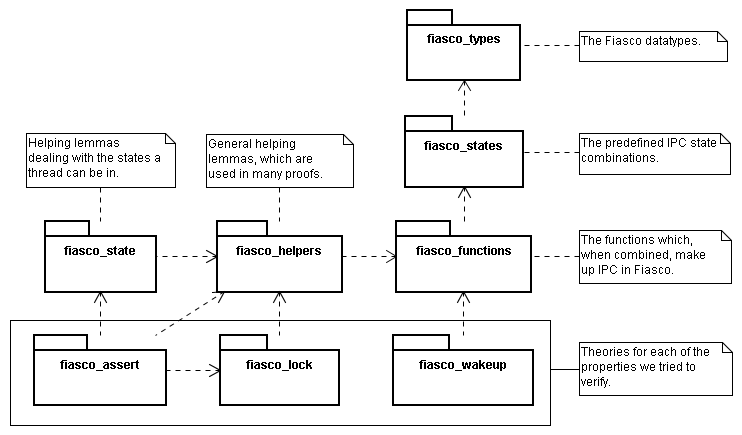
\includegraphics[scale=0.50]{images/diagrams/ipc_class_theories}
\caption{PVS theories structure.}
\end{figure}

The basis is formed by the $<$fiasco\_types$>$ theory, in which the Fiasco-related datatypes (such as threads and timeouts) are defined. These types are used by the $<$fiasco\_functions$>$- and $<$fiasco\_states$>$ theories, where the IPC-related functions and predefined thread states are defined respectively. Having setup the system this way prevents the different theories from redefining these essential IPC components (thus creating a single point of definition). Besides the three theories for our proof properties ($<$fiasco\_assert$>$, $<$fiasco\_lock$>$ and $<$fiasco\_wakeup$>$), there are two theories which define lemmas that are required to verify the properties, but that are not directly related to these properties. The first of these theories is the $<$fiasco\_helpers$>$ theory in which general purpose lemmas are declared. The second assisting theory, $<$fiasco\_state$>$, defines more specific helping lemmas that only involve the state a thread can be in.

\subsection{Fiasco types}
To model the IPC path we have to model the types involved. Because not all details of the types defined in Fiasco are relevant to the properties we want to prove, we do not have to create a one-on-one model. In short, we will only model those types that are directly relevant to the properties we want to prove and on a level sufficiently high enough to be suitable for a proof properties. This means that many Fiasco types will have quite abstract definitions in our models. We will now discuss the types in our PVS model.

\subsubsection{Sender list}
When a sender attempts to send a message to a receiver that is currently busy, that sender is added to the receiver's sender list (which contains all senders wanting to send a message to the receiver). Once the receiver has finished IPC with the current sender, it pops the first sender off the sender list and engages in IPC with that sender (if that sender is still willing to do so).\emptyline

When modeling the sender list, one should note that we abstracted away the receive part as we focused on the send part. Therefore, we were only interested in the sender list from the viewpoint of the sender. Assuming this viewpoint, the status of a receiver's sender list can be one the following options:

\begin{itemize}
 \item The sender is the first item in the sender list and will thus be the next sender with whom the receiver will engage in IPC.
 \item The sender is in the receiver's sender list but not as the first item; that means it will have to wait for the receiver to finish IPC with the preceding senders before IPC can be engaged upon. 
 \item The sender is not enqueued in the sender list at all, which means that it is either currently engaged in IPC with the receiver or not interested in sending a message to the receiver.
\end{itemize}

These options make it clear that the original list-like implementation of the sender list is slightly more complex than it has to be, therefore we modelled the sender list as the following, simple enumeration:

\lstset{language=PVS}
\begin{lstlisting}[caption={PVS: sender list definition.}]
Sender_list: TYPE = {
                      First,    % <this> is the first sender in the list.
                      Enqueued, % <this> is enqueued but not the first item.
                      Dequeued  % <this> is not in the non-empty list.
                    }
\end{lstlisting}

In our model thus every receiver's sender list is specifically targeted to the current active thread.

\subsubsection{Thread state}
Because IPC in Fiasco is very dependent on the states the sender- and receiver are in, the thread state enumeration is one of the key datatypes in our model. In Fiasco, the thread state is stored as a bit mask\footnote{A bit mask is an integer where individual bits are used to store data in.} of all possible states a thread can be in (such as \emph{ready} or \emph{dead}). In PVS we modelled the thread state as a record of boolean values, each one representing a specific state bit being set or not. We could have modelled the bit mask as a PVS bitvector \cite{butler97bitvector}, which would represent the actual implementation more faithfully, but this would have needlessly complicated the model and proof. As we are only interested in which states a thread is in, our simple record of boolean values suffices.

\lstset{language=PVS}
\begin{lstlisting}[caption={PVS: thread state definition.}]
Thread_state: TYPE = [# thread_ready:   bool,
                        thread_cancel:  bool,
                        thread_dead:    bool,
                        thread_busy:    bool,
                        thread_invalid: bool,
                        thread_polling: bool,
                        thread_receiving: bool,
                        thread_ipc_in_progress: bool,
                        thread_send_in_progress: bool,
                        thread_transfer_in_progress: bool #]
\end{lstlisting}

When one compares the definition above with that in the Fiasco source code, one may note that there are some state bits missing in our definition. This is due to the properties we tried to verify, our set of state bits forms the minimal subset of states necessary to create a model in which our properties could be verified. For example, the \emph{thread\_polling\_long} bit is not included in our definition, as it is only used in long IPC which we have not modelled. The \emph{thread\_polling} bit is an example of the importance of the thread state in IPC, as it indicates if a sender is waiting for a receiver to become ready.\emptyline

In Fiasco IPC, there are several predefined states that have specific bits toggled on or off. The main function of these states is to prevent the same states from being redefined each time they are used. An example of such a predefined state is the \emph{Thread\_ipc\_sending\_mask} state, which indicates the state a sender is in when it waits for a receiver to become ready; this state is defined as follows:

\lstset{language=C++}
\begin{lstlisting}[caption={C++: \emph{Thread\_ipc\_sending\_mask} state definition.}]
#define Thread_ipc_sending_mask        (Thread_send_in_progress		| \
					Thread_polling			| \
					Thread_polling_long)
\end{lstlisting}

It is important to note that in the definition above only the three specified bits are sets, the rest is unset. To easily achieve the same effect in our model, we created a basic state, \emph{TS\_empty}, which has all bits unset. Extending this \textit{empty} state allowed us to easily create predefined states such as the one defined above. Our definition of the \emph{Thread\_ipc\_sending\_mask} state is the following:

\lstset{language=PVS}
\begin{lstlisting}[caption={PVS: \emph{Thread\_ipc\_sending\_mask} state definition.}]
TS_ipc_sending_mask: Thread_state = TS_empty WITH [
                                         thread_send_in_progress := true,
                                         thread_polling := true
                                        ]
\end{lstlisting}

We have used a slightly different naming convention, where the \emph{TS}-prefix indicates a thread state definition, for brevity purposes. The \emph{thread\_polling\_long} bit is not included in our predefined state, because it is not part of our model (as explained in more detail earlier).

\subsubsection{Sender and receiver}
When modeling threads, we note that a thread can act as both a sender and a receiver. As threads, senders and receivers are objects containing fields, we naturally defined them as records in our model. For threads to act as a receiver, in Fiasco a thread is an extension of a receiver (it inherits from it). For extension (or inheritance) of records, we used the extensible records mechanism.\emptyline

In Fiasco, a receiver extends a context, which contains many scheduling-related fields (such as the scheduling context). However, as we have abstracted away scheduling, these fields have not made it in our model. The \emph{state} field is not removed from the context though, as is is integral to IPC in Fiasco. A receiver extends a context with two fields of its own. The first of these fields is the \emph{partner} field, which indicates the partner (or sender) thread the receiver is engaged in IPC with. The second field, named \emph{sender\_list}, contains the receiver's sender list, which was discussed earlier.

\lstset{language=PVS}
\begin{lstlisting}[caption={PVS: context, sender and receiver definitions.}]
% The context contains the thread state, here a lot of details have been
% abstracted away which mostly concern scheduling.
Context: TYPE = [# state: Thread_state #]

% The receiver role inherits from <Context> and adds two fields: <partner> and
% <sender_list>. The first reflects the fact that a receiver always has a 
% partner associated with it and the second reflects the threads that want to
% engage in IPC with the receiver.
Receiver: TYPE = Context WITH [# partner: Thread_pointer, 
                                 sender_list: Sender_list #]

% The sender role in our model does not have any real function, but we have
% included it for use in possible later extensions of our model.
Sender: TYPE = [# #]
\end{lstlisting}

Although it might seem odd to include a definition of an empty sender record type, we have included it for use in possible later extensions of our model.

\subsubsection{Thread}
Having modelled the two roles which form the basis of threads, we are now ready to define the threads themselves. Besides the fields from the sender and receiver roles, threads have one additional field, named \emph{thread\_lock}. The function of this field is to model thread locks. This means that every thread can be locked by exactly one other thread. As long as a thread is locked, only the thread owning the lock can access the locked thread. The thread lock itself is defined in Fiasco as a pointer to the thread holding the lock; in our model we have followed this design.

\lstset{language=PVS}
\begin{lstlisting}[caption={PVS: thread definition.}]
% The actual definition of the thread type, which inherits from both the sender
% and the receiver types.
Thread: TYPE = Sender WITH Receiver WITH [# thread_lock: Thread_pointer #]
\end{lstlisting}

To clarify what the result is of using extensible records, we have created an alternative definition of the thread type below, which does not rely on extensible records. The alternative definition results in the same record being created, as both have exactly the same fields.

\lstset{language=PVS}
\begin{lstlisting}[caption={PVS: thread alternative definition.}]
% This alternative thread type definition includes the sender's and receiver's
% fields directly in the definition, it does not use the extensible records
% mechanism, but still has the exact same fields.
Thread: TYPE = [# state:   Thread_state,
                  partner: Thread_pointer,
                  sender_list: Sender_list,
                  thread_lock: Thread_pointer #]
\end{lstlisting}

For the thread pointer type, we have followed the C++ implementation where pointers are just integers (referring to objects). As explained, the thread lock was modelled as a pointer to the thread owning the lock. However, it is also possible that there is no thread lock on a thread. In Fiasco, this is implemented by having the thread lock being equal to the NULL-pointer. We modelled the NULL-pointer as a thread pointer instance without a specific value. One might expect the zero thread to have the value zero (corresponding to the C++ implementation), but then changing the type of a thread pointer to a positive number would also require the definition of the zero thread to be changed (which would not be necessary with our definition).

\lstset{language=PVS}
\begin{lstlisting}[caption={PVS: thread pointer definition.}]
% A pointer to a thread is just an integer, this reflects a C++ pointer also
% being an integer.
Thread_pointer: TYPE = int

% Define the zero thread pointer, which represents the C++ NULL pointer.
Zero_thread: Thread_pointer
\end{lstlisting}

\subsubsection{Threads}
In Fiasco, at any single time there can (and probably will be) more than one created thread. For each created thread, there exists a pointer to access that thread. There is also a subset of threads, called the ready-list, which contains all threads ready to be scheduled (with some exceptions, see the backgrounds on Fiasco). However, as scheduling has not been incorporated in our model, the ready-list has also been abstracted away. The only thing for us to model is thus the list of created threads, which we have defined as a function from thread pointers to threads.

\lstset{language=PVS}
\begin{lstlisting}[caption={PVS: definition of thread list.}]
% The thread list is a function which translates thread pointers to threads;
% this reflects the C++ concept of pointers to objects (in this case pointers
% to threads).
Thread_list: TYPE = [Thread_pointer -> Thread]
\end{lstlisting}

\subsubsection{Other types}
Many functions involved in the IPC path return an IPC error code. Although there are many possible error codes that can be returned, the source code only checks \textit{if} an error occured and is not interested in the actual error code itself\footnote{The reason why there are still many different error codes is that the caller of IPC might be interested in what went wrong.}. We have therefore chosen to model the error codes as a boolean value which indicates whether an error occured or not. A similar reasoning can be applied to IPC timeouts. We are only interested \textit{if} a timeout occured and not \textit{how}. Timeouts are thus also a defined as a boolean value.

\lstset{language=PVS}
\begin{lstlisting}[caption={PVS: IPC error codes- and timeout definitions.}]
% Most functions in Fiasco return an error code, of which there are many.
% However, we are only interested in whether an error occured and thus the
% error code is modelled as a boolean value.
Ipc_err: TYPE = bool

% Indicates if a timeout occured, additional details of timeouts such as 
% the exact time at which they expire are not of interest to us.
L4_timeout: TYPE = bool
\end{lstlisting}

\subsection{Fiasco functions}

\subsubsection{Converting from sequential- to functional code}
One of the key design issues was how to model the execution of imperative C++ source code in the functional language used by PVS. Because our model should represent the Fiasco C++ source, we have tried to remain very close to the source code in our conversion to PVS. This resulted in our PVS model quite often directly reflecting the C++ source, which allows anyone familiar with the Fiasco sources to quickly grasp the inner workings of our model. Another benefit of this strict adherence to the source code, is an added confidence in our model as one can easily check if the model accurately reflects the source code. To create this fairly direct conversion, we often used the \emph{LET} construction, which can be used to update data without transferring control to another function. Conveniently, most flow-control structures (such as \emph{if}-statements) could be directly translated to PVS.\emptyline

Functions defined in C++ can have \emph{side-effects}, which means that functions can modify some global state besides modifying their return values. We therefore introduced the concept of a system state in our model, which each function should be able to access and modify. This is achieved by having each function take the system state as one of its input parameters and also have it return the system state. An example of this method is shown below, where the \emph{sys\_thread\_ex\_regs()} function takes a parameter of the type \emph{System\_state} (which definition will be discussed shortly) and returns the original system state, but with the \emph{thread\_cancel} bit of the thread pointed to by \emph{tp} set to true.

\lstset{language=PVS}
\begin{lstlisting}[caption={PVS: an example of a system state-modifying function.}]
sys_thread_ex_regs(tp: Thread_pointer,state_old: System_state): System_state =
  state_old WITH [(threads)(tp)`state`thread_cancel := true]
\end{lstlisting}

\subsubsection{System state}
Now that we have a way to simulate the updating of the system state, we have to look at what fields the system state should contain. As the list of created threads should be accessible at all times, it has to be included into the system state. Furthermore, in our proofs we will be looking at IPC from the viewpoint of a single thread, in our case the active, running thread\footnote{In Fiasco there can only be one thread running at any single moment in time, support for multi-processor systems has not yet been integrated into the kernel. Consequently, in a multi-processor system, Fiasco will only use one of those processors.}, which we will refer to as the \emph{this} thread (with a clear analogy to the corresponding C++ term). A better name for the \emph{this} field would have been \emph{this\_pointer}, but we favored the shorter version for brevity purposes. This leads to the following, preliminary system state:

\lstset{language=PVS}
\begin{lstlisting}[caption={PVS: incomplete system state, focusing on threads.}]
System_state: TYPE = 
            [# 
              this:    Thread_pointer, % Pointer to active thread.
              threads: Thread_list     % List of all threads.
            #]
\end{lstlisting}

It is now possible to access the \emph{this} thread by providing it as a parameter to the \emph{threads} field (which is actually a function from thread pointers to threads). In our model, most proofs will involve the \emph{this} thread as that is the thread from which viewpoint we look at IPC.

\lstset{language=PVS}
\begin{lstlisting}[caption={PVS: example of accessing this thread.}]
% Return the this thread, which the <this> field of the system state points to.
get_this_thread(state: System_state): Thread = 
  state`threads(state`this)
\end{lstlisting}

There is a problem with the current system state definition though. As it is defined now, it is possible that the current, running thread is the zero thread (pointed to by the NULL-pointer), which is obviously incorrect. To correct this flaw, the type of the \emph{this} field was changed to the \emph{This\_thread\_pointer} type, which is defined as the subset of thread pointers not equal to the zero thread:

\lstset{language=PVS}
\begin{lstlisting}[caption={PVS: definition of special this pointer type.}]
% The pointer to the current active thread (the <this> thread) must never be
% the <Zero_thread> (as it points to nothing) and thus we have defined
% a special type of thread pointer for the <this> thread which excludes the
% thread pointer being equal to the <Zero_thread>.
This_thread_pointer: TYPE = { tp: Thread_pointer | NOT tp = Zero_thread }
\end{lstlisting}

\subsubsection{Errors and timeouts}
One of the problems we encountered when converting from C++ to our model, were the varying return values of the functions involved in IPC. Each IPC-related function in Fiasco had one of the following three return types: \emph{void}\footnote{Which indicates no value is returned.}, \emph{bool} or \emph{Ipc\_err}. A closer inspection revealed that all bool-returning functions did not have any side-effects (with one exception discussed later), whereas the other functions did. As we explained earlier, a state-modifying function (one with side-effects) must at least return the updated system state. As the functions returning an \emph{Ipc\_err} value also modified the system state, those functions should return the updated system state, but they also had to return the error value. One option was to have each function return a tuple of a system state and an error value. However, as there are only a couple of functions modifying the error value, we opted for another solution: integration of the error code into the system state:

\lstset{language=PVS}
\begin{lstlisting}[caption={PVS: incomplete system state, with integrated error field.}]
System_state: TYPE = 
            [# 
              this:    This_thread_pointer, % Pointer to active thread.
              threads: Thread_list,         % List of all threads.
              error:   Ipc_err              % Indicates if error occurred.
            #]
\end{lstlisting}

The initial system state has the \emph{error} field set to false, which makes sense as no error can have occured \textit{before} IPC has even been started. While engaged in IPC, this field can be set by functions to indicate if an error occured; this value can subsequently be checked by the caller of the function to see if an error was returned. Most often it was not necessary for the caller of the error-returning function to reset the \emph{error} field to false after an error was returned, as an error often resulted in IPC being prematurely aborted. An example of this is shown in the code excerpt below, where the \emph{do\_ipc\_send\_part()} function calls \emph{try\_handshake\_receiver()}. The latter sets the \emph{error} field to true when the partner is invalid and then immediately returns; the \emph{do\_ipc\_send\_part()} function then checks if the \emph{error} field has been set to true and acts accordingly (by immediately returning from the function):

\lstset{language=PVS}
\begin{lstlisting}[caption={PVS: example of error setting and checking.}]
% Try to have the sender and receiver agree upon engaging in IPC.
try_handshake_receiver(partner: Thread_pointer, 
                       state_old: System_state): System_state =
  % Immediately return with an error if the partner is invalid.
  IF partner = Zero_thread OR [...] THEN
    state_old WITH [error := true]
  ELSE
    [...]
  ENDIF

% Handle the send part in the do_ipc() function.
do_ipc_send_part(partner: Thread_pointer, have_receive: bool, 
                 state_old: System_state): System_state =
  % Start with a handshake and immediately return if an error occured.
  LET state_temp = try_handshake_receiver(partner,state_old) IN
  IF state_temp`error THEN
    state_temp   
  ELSE 
    [...]
  ENDIF
\end{lstlisting}

Following a similar line of reasoning, we integrated a \emph{timeout} field into the system state, which indicates if a timeout has occured. Once again, this field is initially set to false and only becomes true when a timeout occured. Our basic system state is thus defined as follows:

\lstset{language=PVS}
\begin{lstlisting}[caption={PVS: basic system state, with integrated \emph{timeout} field.}]
System_state: TYPE = 
            [# 
              this:    This_thread_pointer, % Pointer to active thread.
              threads: Thread_list,         % List of all threads.
              error:   Ipc_err,             % Indicates if error occurred.
              timeout: L4_timeout           % Indicates if timeout occurred.
            #]
\end{lstlisting}

To ensure that initially the \emph{error}- and \emph{timeout} fields are set to false, both fields are explicitly unset at the start of the IPC path (which is the \emph{sys\_ipc()} function). Where possible though, we have not made any assumptions about the initial values of fields or parameters to keep the model as generic as possible:

\lstset{language=PVS}
\begin{lstlisting}[caption={PVS: system state initialization in the \emph{sys\_ipc()} function.}]
sys_ipc(have_send: bool, partner: Thread_pointer,
        have_receive: bool, sender: Thread_pointer,
        state_old: System_state): System_state = 
  LET state_temp = state_old WITH [(error)   := false,
                                   (timeout) := false]
  IN
    % Make sure there is either a send- or receive part, if so start IPC.
    IF have_send OR have_receive THEN
      do_ipc(have_send,partner,have_receive,sender,state_temp)
    ELSE
      state_temp WITH [(error) := true]
    ENDIF
\end{lstlisting}

One can cleary see that IPC is only started when there is a send and/or receive part (which makes sense as otherwise there is nothing to do).

\subsubsection{Increment model development}
As said, we have developed our model incrementally. We will illustrate this with an example. Initially, we defined the \emph{sender\_ok()} function as follows:

\lstset{language=PVS}
\begin{lstlisting}[caption={PVS: \emph{sender\_ok()} function without implementation.}]
% Indicates if a partner is ready for a sender.
sender_ok(sender: Thread_pointer, receiver: Thread_pointer,
          state_old: System_state): bool 
\end{lstlisting}

This function is defined without an implementation, which means that PVS cannot determine the value returned by the function when it is called; any use of this function in a proof therefore requires all possible return values (in this case only two: \emph{true} or \emph{false}) to be checked. Using unimplemented functions, we were able to rapidly develop a very crude model. After we were satisfied with the general structure of the model, we added implementations to the unimplemented functions to have them better reflect the source code. The definition of the \emph{sender\_ok()} function \textit{with} implementation is listed below.

\lstset{language=PVS}
\begin{lstlisting}[caption={PVS: \emph{sender\_ok()} function.}]
% Indicates if a partner is ready for a sender.
sender_ok(sender: Thread_pointer, receiver: Thread_pointer,
          state_old: System_state): bool =
  % The receiver should at least be in a receiving IPC state.
  IF NOT state_old`threads(receiver)`state`thread_receiving OR
     NOT state_old`threads(receiver)`state`thread_ipc_in_progress
  THEN
    false
  % Open wait: no partner should be specified and the sender should be the 
  % first in the receiver's sender list.
  ELSIF state_old`threads(receiver)`partner = Zero_thread AND
        state_old`threads(receiver)`sender_list = First THEN 
    true
  % Closed wait: check if the sender is the same as the partner specified.
  ELSIF sender = state_old`threads(receiver)`partner THEN
    true
  ELSE
    false
  ENDIF
\end{lstlisting}

We have already discussed shortly how we converted from the Fiasco C++ source to PVS. To show an example of such a conversion, we have included the \emph{sender\_ok()} function as defined in Fiasco, which can be compared to our PVS definition listed above.

\lstset{language=C++}
\begin{lstlisting}[caption={C++: \emph{sender\_ok()} function.}]
bool Receiver::sender_ok (const Sender *sender) const
{
  unsigned ipc_state = state() & (Thread_receiving |
                                  //                 Thread_send_in_progress |
                                  Thread_ipc_in_progress);

  // If Thread_send_in_progress is still set, we're still in the send phase
  if (EXPECT_FALSE (ipc_state != (Thread_receiving | Thread_ipc_in_progress)))
    return false;

  // Check open wait; test if this sender is really the first in queue
  if (EXPECT_TRUE(!partner()
                  && (!_sender_first || sender == _sender_first))) 
    return true;

  // Check closed wait; test if this sender is really who we specified
  if (EXPECT_TRUE (sender == partner()))
    return true;

  return false;
}
\end{lstlisting}

\subsection{Splitting functions}
Three of Fiasco's functions have been split into several functions in our PVS model, namely the \emph{do\_ipc()}, \emph{do\_send\_wait()} and \emph{ipc\_receiver\_ready()} functions. Although the splitting is not in accordance with our aim to create a (mostly) one-on-one conversion of the source code, for each split there is a good reason. The reason why the \emph{do\_ipc()} function was split in two parts was to separate the send part from the receive part. This enabled us to do proofs for only one of the two parts, thus creating more compact and modular proofs (a change in the receive part would not affect proofs of the send part\footnote{This is due to the fact that the receive part is always executed \textit{after} the send part and thus cannot influence it. The reverse does not automatically hold, as the receive part \textit{can} be preceded by a send part which could influence its begin state.}). The main incentive to split the \emph{do\_send\_wait()} function was its considerable size. Splitting once again resulted in more modular and compact proofs. The last function, \emph{ipc\_receiver\_ready()}, was split for a totally different reason. In our model, we differentiate between functions that modify the system state and those that do not. The former always return the system state, whereas the latter return anything but the system state (for example boolean values). The problem with the \emph{ipc\_receiver\_ready()} function was that it had to both modify the system state and return a boolean value. Therefore, the function was split into a state-modifying part (the \emph{ipc\_receiver\_ready\_change()} function) and a boolean-returning part (\emph{ipc\_receiver\_ready()}). The state-modification only occurs when the \emph{ipc\_receiver\_ready()} function returns true, so in our model a return value of true results in calling the \emph{ipc\_receiver\_ready\_change()}.

\lstset{language=PVS}
\begin{lstlisting}[caption={PVS: calling the split \emph{ipc\_receiver\_ready()} function.}]
% Check if the sender is ready for the receiver.
IF ipc_receiver_ready(sender,receiver,state_old)
THEN
  % Apply the changes caused by the side-effects of the 
  % ipc_receiver_ready() function.
  ipc_receiver_ready_change(sender,receiver,state_old)
ELSE
  state_old
ENDIF
\end{lstlisting}

An overview of the functions split and the functions into which they were split is listed below:

\begin{table}[!htc]
\begin{tabular}{ll}
\textbf{Original function} & \textbf{Split into} \\
\hline
\emph{do\_ipc()} & \emph{do\_ipc\_send\_part()}, \emph{do\_ipc\_receive\_part()} \\
\emph{do\_send\_wait()} & \emph{do\_send\_wait()}, \emph{do\_send\_wait\_loop()}, \emph{do\_send\_wait\_finish(}) \\
\emph{ipc\_receiver\_ready()} & \emph{ipc\_receiver\_ready()}, \emph{ipc\_receiver\_ready\_change()} \\
\hline
\end{tabular}
\caption{Model: split functions.}
\end{table}

\subsection{Preemption points}
As explained in detail earlier, in Fiasco a preemption point is a function that temporarily allows other threads to be scheduled and executed in favor of the current executing thread. When another thread indeed gets scheduled, its execution might change the system state. In our model a preemption point is thus a state-modifying function. Because we have abstracted away scheduling, we have to simulate the result of the scheduling on the system state. Our focus is thus on \textit{what} the result of a preemption point on the system state is, not on \textit{how} this result is achieved. In our model, we discern between five different actions that can occur in a preemption point:
\begin{itemize}	
 \item Nothing happens.
 \item The partner thread is killed (through the \emph{kill()} function).
 \item An IPC timeout occurs.
 \item The ongoing IPC is cancelled (through the \emph{sys\_thread\_ex\_regs()} function).
 \item The receiver becomes ready to receive a message from the sender.
\end{itemize}

These five actions are not complete though, one of the most striking omissions is a concurrent sender wanting to send a message to the same receiver. We have modelled only the five actions listed above to keep the model compact, more actions would further complicate the model and proofs.\emptyline.

Even though the first of the five actions is the most likely to occur, we will model the actions as if they all have the same probability. This simplified version of the real situation does not have any negative effect on the validity of the model, all possible actions have to be examined in a proof anyway. The possible preemption actions are defined as the enumeration type \emph{Preemption\_action}. Although the enumeration might suggest otherwise, a single preemption point might in fact execute several of its possible actions. Therefore, we have also created the \emph{Preemption\_actions} type, which is just a list of preemption actions.

\lstset{language=PVS}
\begin{lstlisting}[caption={PVS: \emph{preemption\_action} type.}]
% Enumeration of the possible preemption actions.
Preemption_action: TYPE = {
                            Nothing,            % Nothing happens.
                            Kill,               % The partner is killed.
                            Timeout,            % A timeout occurs.
                            Sys_thread_ex_regs, % IPC is cancelled.
                            Receiver_ready      % The receiver becomes ready.
                          }
                          
Preemption_actions: TYPE = list[Preemption_action]
\end{lstlisting}

\subsubsection{Randomness}
When executing a preemption point, one never knows beforehand what actions it will execute, its behaviour appears to be random. One of our main problems was how to model this randomness. Although PVS has the \emph{choose()} function, which randomly chooses an element from a set, we could not use it in our model. The problem with this function is due to the very definition of a function: equal input results in equal output. In our case, its input would always be equal to the set of possible combinations of preemption actions (its powerset). Because there are several calls to the preemption point function, each of which has to use the same \emph{choose()} function call, the returned actions would in each case be the same. To circumvent this, we created an uninterpreted function, named \emph{preemption\_action()}, which returns a list of preemption actions. As the function contains no implementation, the output is essentially random. To prevent the problem with equal inputs, the \emph{preemption\_action()} function accepts a single input parameter, which we make sure is different with each call.

\lstset{language=PVS}
\begin{lstlisting}[caption={PVS: \emph{preemption\_action()} function.}]
% Return a (random) preemption action.
preemption_action(n: nat): Preemption_actions
\end{lstlisting}

To allow the seed input parameter\footnote{A value which only function is to randomize behaviour is often referred to as a seed value.} to be different with each call, a \emph{seed} field was added to the system state:
\lstset{language=PVS}
\begin{lstlisting}[caption={PVS: expanded system state, with added \emph{seed} field.}]
% Modified system state with added <seed> field.
System_state: TYPE = 
            [# 
              this:    This_thread_pointer, % Pointer to active thread.
              threads: Thread_list,         % List of all threads.
              error:   Ipc_err,             % Indicates if error occurred.
              timeout: L4_timeout,          % Indicates if timeout occurred.
              seed:    nat                  % Seed used for randomness.
            #]
\end{lstlisting}

Before each call to the \emph{preemption\_action()} function, the seed is incremented to ensure its uniqueness. After a list of preemption actions has been retrieved, what remains is to execute those actions. Precisely that is the function of the \emph{preemption\_point\_actions()} function, it executes each action and updates the system state correspondingly. The \emph{preemption\_point()} function is defined as follows:

\lstset{language=PVS}
\begin{lstlisting}[caption={PVS: \emph{preemption\_point()} function.}]
preemption_point(partner: Thread_pointer, allow_timeout: bool, 
                 state_old: System_state): System_state =
  LET 
    % Increment the seed and use it to get a random list of preemption 
    % actions.
    state_old = state_old WITH [seed := state_old`seed + 1],
    actions = preemption_action(state_old`seed)
 IN
    % Execute the preemption actions.
    preemption_point_actions(actions,partner,allow_timeout,state_old)
\end{lstlisting}

We see that the \emph{preemption\_point()} function not only takes the system state as one of its parameters, but also a boolean value named \emph{allow\_timeout}. The function of this value is to indicate if a timeout can occur in the preemption point, which is not always so because timeouts are only used in some functions (such as the \emph{do\_send\_wait()} function).

\subsubsection{Preemption actions}
For execution of the randomly chosen preemption actions, the \emph{preemption\_point\_actions()} function is used. The definition of this function is very simple. It takes the same parameters as the \emph{preemption\_point()} function calling it, but with one additional parameter that specifies the preemption actions to be executed. As a reminder, the \emph{Preemption\_actions} type is actually a list of \emph{Preemption\_action} instances. The \emph{preemption\_point\_actions()} function first checks if the action list is empty, if so the system state is returned unmodified. If the list is not empty, the system checks which action it should execute and then updates the system state accordingly. It then continues executing the remaining actions until there are no actions left; the function is therefore (defined as) a recursive function\footnote{A recursive function calls itself.}.

\lstset{language=PVS}
\begin{lstlisting}[caption={PVS: \emph{preemption\_point\_actions()} function.}]
% Execute a list of preemption point actions.
preemption_point_actions(actions: Preemption_actions, partner: Thread_pointer,
                         allow_timeout: bool, 
                         state_old: System_state): RECURSIVE System_state =
  CASES actions OF
    null: state_old,
    cons(action,remaining_actions):
    LET state_temp = 
      % Check if a call was made to sys_thread_ex_regs().
      IF action = Sys_thread_ex_regs THEN
        sys_thread_ex_regs(state_old`this,state_old)
      % Only allow a timeout to occur when specified, most of the time a 
      % timeout cannot occur.
      ELSIF action = Timeout AND allow_timeout THEN
        timeout(state_old`this,state_old)
      % Check if the partner is killed.
      ELSIF action = Kill THEN
        kill(partner,state_old)
      % A receiver can only become ready when it is not equal to the sender,
      % if so it would be waiting forever.
      ELSIF action = Receiver_ready THEN
        receiver_ready(state_old`this,partner,state_old)
      ELSE
        state_old
      ENDIF
    IN
    % Execute the remaining actions.
    preemption_point_actions(remaining_actions,partner,allow_timeout,state_temp)
  ENDCASES
  MEASURE length(actions)
\end{lstlisting}

Most of these functions have very simple definitions, with the notable exception of the \emph{receiver\_ready()} function. As detailed earlier, the \emph{receiver\_ready()} function models a receiver becoming ready to receive a message from the sender; we are in fact modeling that the receiver is executing the receive part of IPC. A receiver becomes ready for a sender in its receiving loop, which is preceded by the necessary initialization. To prevent this initialization from occuring several times, we created a slightly modified version of the receive part in our \emph{receiver\_ready()} function, which uses a newly added \emph{receiver\_initialized} system state field; initially this field is set to false to guarantee that the receiver will always be initialized.\emptyline

Another problem with the \emph{receiver\_ready()} lies in it calling \emph{ipc\_receiver\_ready()}, which is a boolean-returning function with side-effects; the solution to this problem has been discussed earlier. We will now list the definition of the \emph{receiver\_ready()} function:

\lstset{language=PVS}
\begin{lstlisting}[caption={PVS: \emph{ipc\_receiver\_ready()} function.}]
% This preemption action signifies a receiver becoming ready to receive a 
% message from a sender.
receiver_ready(sender: Thread_pointer, receiver: Thread_pointer,
               state_old: System_state): System_state = 
  LET
    state_old = 
      % Check if the receiver has been initialized.
      IF NOT state_old`receiver_initialized THEN 
        % Prepare the receiver using a 'random' partner.
        prepare_receive_dirty(Receiver_partner_thread,receiver,state_old)
          WITH [(receiver_initialized) := true]
      ELSE
        state_old
      ENDIF
  IN
  % Make sure the receiver is in the right state to receive from a sender.
  IF state_old`threads(receiver)`state`thread_receiving AND
     state_old`threads(receiver)`state`thread_ipc_in_progress AND NOT
     state_old`threads(receiver)`state`thread_cancel
  THEN
    % Closed wait: check if the sender is the same as the partner specified.
    IF sender = state_old`threads(receiver)`partner THEN
      % Check if the sender meets the conditions of the receiver
      IF in_sender_list(receiver,state_old) AND 
         ipc_receiver_ready(sender,receiver,state_old)
      THEN
        % Apply the changes caused by the side-effects of the 
        % ipc_receiver_ready() function.
        ipc_receiver_ready_change(sender,receiver,state_old)
      ELSE
        state_old
      ENDIF
    % Open wait: no partner should be specified and the sender should be 
    % the first item.
    ELSE
      % Check if the sender is not ready in which case it should be removed
      % from the sender list.
      IF NOT ipc_receiver_ready(sender,receiver,state_old) THEN
        sender_dequeue_head(receiver,state_old)
      ELSE
        % Apply the changes caused by the side-effects of the
        % ipc_receiver_ready() function.
        ipc_receiver_ready_change(sender,receiver,state_old)
      ENDIF
    ENDIF    
  ELSE
    state_old
  ENDIF
\end{lstlisting}